\section{Result Ownership at the Tool Boundary}
\label{sec:ownership}

Section~\ref{sec:certify} established which calls are reusable. Q3 asks where a reused result should live. This
section is a case study on the E-eval subset of the assumption-based tier. It compares designs that admit the same
calls and save the same execution, and that differ only in who holds the bytes.

% Fig. 4 -- ownership (column width, Section 6)
\begin{figure}[htbp]
  \centering
  \subcaptionbox{Tool-boundary result ownership and the lifetime of a shared object\label{fig:designs}}{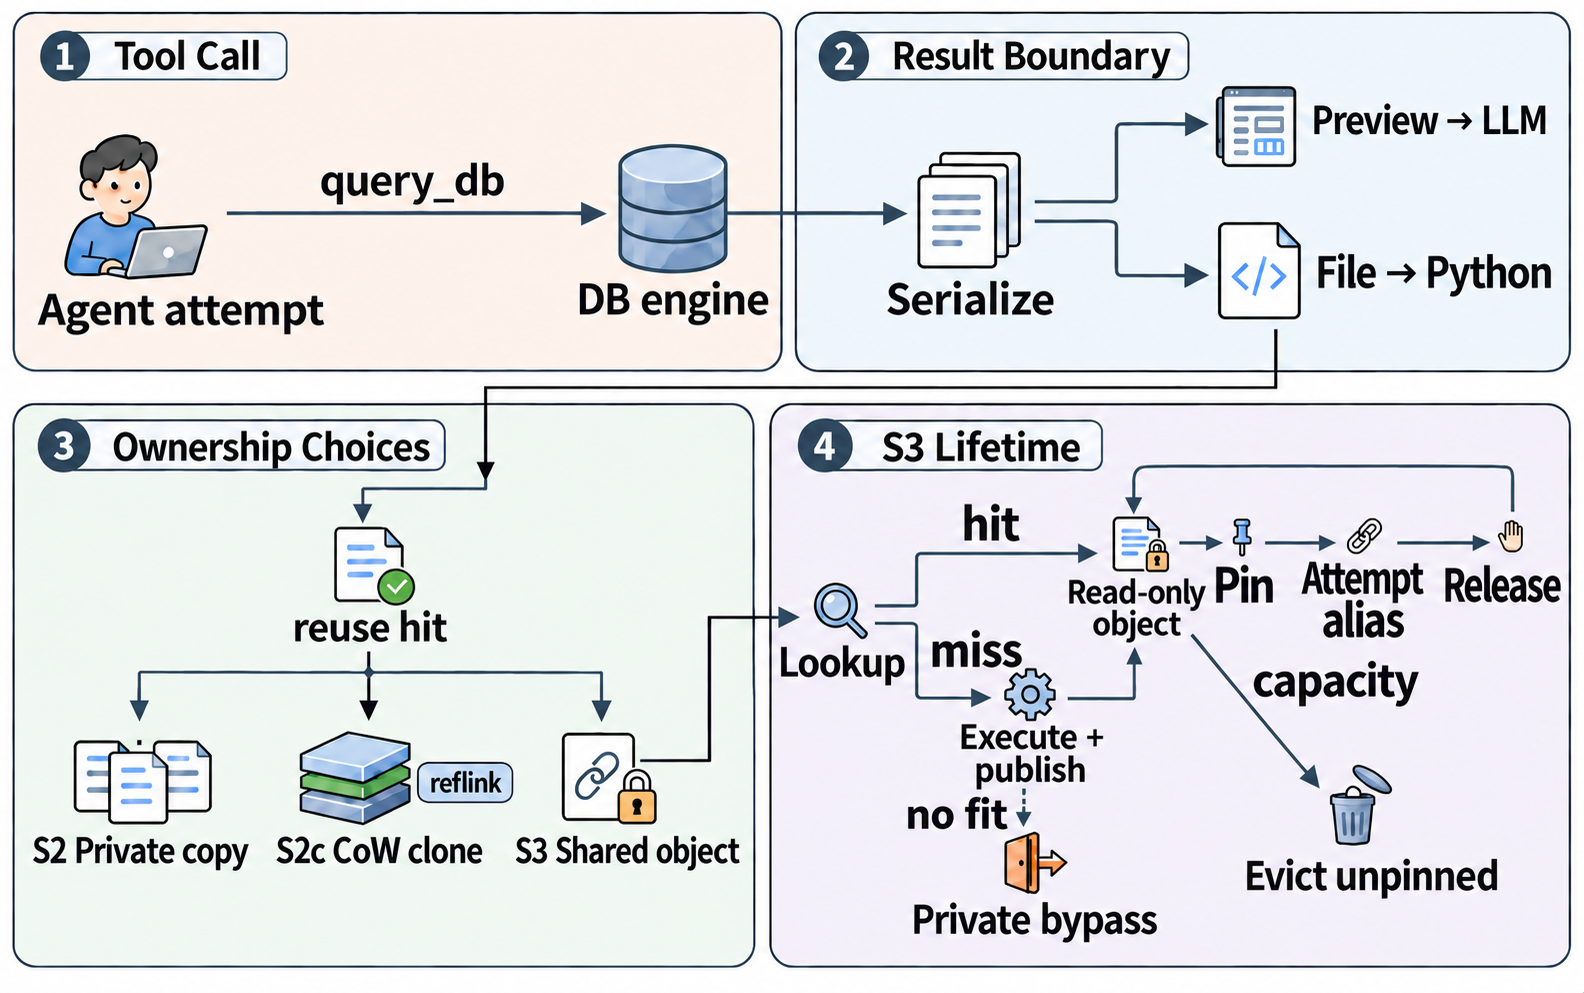
\includegraphics[width=\columnwidth]{figures/fig4a_ownership}}\\[3pt]
  \subcaptionbox{Footprint vs.\ $N$\label{fig:footN}}{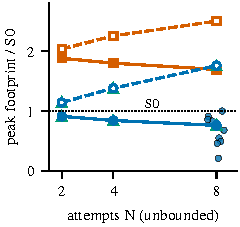
\includegraphics[height=1.45in]{figures/fig4b_footprint_N}}\hfill
  \subcaptionbox{Footprint vs.\ budget\label{fig:footB}}{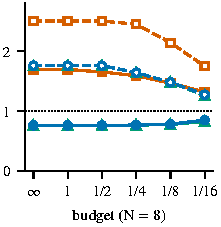
\includegraphics[height=1.45in]{figures/fig4c_footprint_budget}}\\[1pt]
  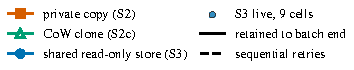
\includegraphics{figures/fig4_legend}
  \caption{Result ownership decides storage cost. (a) A \texttt{query\_db} result is serialized into an LLM preview and a file for Python. Only the file takes part in ownership. On a hit, S2 provides a private copy and S2c a reflink clone. S3 aliases one shared read-only object. SD is omitted because it changes execution but retains attempt-private serialization and files. Section~\ref{sec:designs} describes the lifetime of an S3 object. (b, c) Simulated peak footprint relative to no sharing (S0) on the assumption-based E-eval subset. Values are medians over the 52 tasks with nonzero S0 footprint (50 resamples). Panel (b) uses an unbounded budget and panel (c) uses $N=8$.
  Solid lines retain outputs to batch end, and dashed lines are sequential retries. Dots in (b) are live S3/S0 on the
  9 calibration cells with admitted spilled bytes ($N=8$, unbounded budget, median of 5 resamples, jittered). The
  simulator reproduces each cell.}
  \label{fig:ownership}
  \Description{Top: a four-region diagram. Region 1 shows an agent attempt calling query_db on a database engine. Region 2 shows the result serialized into a preview for the LLM and a file for Python. Region 3 shows three ownership choices on a reuse hit: a private copy, a copy-on-write clone, and a shared object. Region 4 shows the lifetime of a shared object: lookup, hit or miss with execute and publish, pin, attempt alias, release, eviction of unpinned objects under capacity pressure, and a private bypass when a result does not fit. Bottom: two line plots of peak footprint relative to no sharing. Private copies stay above 1, the shared store and clones stay near 0.76 to 0.91 when outputs are retained and between 1.14 and 1.76 for sequential retries.}
\end{figure}


\subsection{Design Space}
\label{sec:designs}

All six designs keep the format of DAB's tool messages and bindings (Figure~\ref{fig:designs}). \emph{S0 Isolated}
executes every call. \emph{S1 Session memo} reuses results within an attempt. \emph{SD} is an execution-only cache
model that caches results inside the engine, as warehouse result caches do
\cite{snowflake2026persisted,google2026bqcache,databricks2026querycache}. A hit skips execution, and every attempt
still serializes the result and writes and keeps its own file. \emph{S2 Private copy} keeps one cached copy of each
result per batch and gives every attempt that hits a private copy of the file. \emph{S2c CoW clone} does the same
with copy-on-write clones that share extents through reflink \cite{rodeh2013btrfs}. \emph{S3 Shared read-only store}
keeps one read-only file per result in a store shared by the batch. It binds an attempt-local alias, a symbolic link,
to that file. 

\paragraph{Shared-store protocol.}
A \emph{lookup} under the store's lock finds the key and moves it to the most-recently-used end. It increments the
key's reference count once per attempt and binds the alias or the inline value. On a \emph{miss}, the attempt
executes and serializes the query. To \emph{publish}, it makes room by evicting least-recently-used objects whose
reference count is zero. It then makes the file read-only and inserts it. If nothing evictable frees enough space,
the result \emph{bypasses} the store and is written as a private file. The attempt's references are \emph{released}
when the attempt ends under the sequential lifetime, or when the batch ends under the retained lifetime. Under
concurrency, a miss follows one of two policies. It executes optimistically and re-checks the table before
publishing, discarding its own copy if another attempt published first. Alternatively it waits for the attempt
already executing that key (\emph{single-flight}).

\paragraph{Design rationale.}
Aliases instead of copies avoid writing a result once per hit. Clones avoid the write too but need a file system with reflink \cite{mkfsxfs2026}. The node-local XFS file systems of our cluster offer reflink, and its GPFS scratch file system does not. Read-only objects keep one attempt's code from accidentally altering a result another attempt reads. Private copies remain writable by design. Pinning keeps eviction from deleting an object behind a
live alias (Section~\ref{sec:concurrency}). Footprint depends on how long outputs live, so we report two lifetimes.
Under the \emph{retained} lifetime, every attempt's outputs stay readable until the batch ends, and S3 holds its
references until then. Under the \emph{sequential} lifetime, attempt-private files are deleted and S3 references
dropped when an attempt ends. Budgets are fractions of a task's distinct admitted stored bytes over all of its runs.
This base depends neither on $N$ nor on the sampled batch. Its median over tasks is 17.4\,MB and its 95th percentile
13.7\,GB.

% Table 2 -- designs (full width)
\begin{table*}[tbp]
  \caption{Reuse designs at $N=8$ with an unbounded budget on the assumption-based E-eval subset (simulation, 50
  resamples). DB-execution saving relative to S0 is the median over 54 tasks. Bytes written and peak footprint
  relative to S0 are medians over the 52 tasks with nonzero S0 writes, under the retained and sequential lifetimes of
  Section~\ref{sec:designs}. Both are exact accounting. Modeled tool-time saving is the simulator's estimate (median
  over 54 tasks), with a per-run error of 43.9\% on this subset. The live calibration
  compares S2, S2c and S3, and SD's tool time is modeled only. Measured primitives are the live copy rate per byte
  (258 copies) and the clone (482) and alias (282) times.}
  \label{tab:designs}
  \small
  \begin{tabular}{@{}lrrrrlr@{}}
\toprule
 & DB-time & Written & \multicolumn{2}{c}{Footprint / S0} & Measured & Modeled tool-time \\
\cmidrule(lr){4-5}
Design & saving \% & / S0 & retained & sequential & primitive & saving \% \\
\midrule
Isolated (S0) & 0.0 & 1.00 & 1.00 & 1.00 & --- & 0.0 \\
Session memo (S1) & 3.4 & 0.98 & 0.98 & 0.96 & --- & 3.4 \\
Execution-only cache model (SD) & 24.5 & 1.00 & 1.00 & 1.00 & --- & 11.8 \\
Private copy (S2) & 24.5 & 1.70 & 1.70 & 2.50 & copy 0.46 ns/B & 24.9 \\
CoW clone (S2c) & 24.5 & 0.76 & 0.76 & 1.76 & clone 0.29 ms & 24.8 \\
Shared read-only store (S3) & 24.5 & 0.76 & 0.76 & 1.76 & alias 12.6\,\textmu s & 25.0 \\
\bottomrule
\end{tabular}

\end{table*}


\subsection{Storage and Time Costs}
\label{sec:storage}

Table~\ref{tab:designs} compares the designs at $N=8$ with an unbounded budget. Every cross-attempt design skips the
same executions and saves 24.5\% of the median task's DB-execution time. The designs differ in what happens to the
result file. In the simulator's tool-time model, the three tool-boundary caches (S2, S2c, S3) save 24.8--25.0\% and
the execution-only model 11.8\%. A hit in the engine still pays serialization and the file write, and the live
comparison of tool time follows below. Storage separates the designs, and its accounting is exact. Private copies
write 1.70$\times$ the bytes of no sharing, since every hit writes a copy, while S2c and S3 write 0.76$\times$. Per
task, S3 writes 0.448$\times$ the bytes of S2 at $N=8$ (95\% CI 0.433--0.459 over the 52 tasks with spilled results).
The ratio is 0.489$\times$ at $N=2$ and 0.336$\times$ at $N=50$, at a simulated tool-time ratio of 0.999. Per engine,
S3 writes at most 0.63$\times$ the bytes of S2 at every $N$ and budget.

Figures~\ref{fig:footN} and~\ref{fig:footB} show the footprint. With outputs retained to the batch end, S3 and S2c
store 0.91$\times$ of no sharing at $N=2$ and 0.76$\times$ at $N=8$, while S2 stores 1.70$\times$. The live runs
measure this footprint directly at the unbounded budget, where nothing is evicted and the reference lifetime cannot
matter. On the 9 calibration cells with admitted spilled bytes, S3 stores 0.68$\times$ of S0 (range 0.21--1.00) and
S2 1.55$\times$. These values equal the simulator cell by cell, and on-disk size matches the accounting in all 180 runs. Under the sequential lifetime S2, S2c and S3 store more than no sharing, because cached results
outlive the attempt that produced them. S3 still stores 25--44\% less than S2, and the budget bounds the excess
(1.27$\times$ of S0 at 1/16).

In our copy-on-write accounting, S2c matches S3 in bytes and footprint. The median per-task ratio of S3 to S2c is 1.000 at every $N$ and budget except the tightest retained one (1/16). There it reaches 1.0029 at $N=8$. In tool
time S3 is slightly ahead, at 0.997--0.999 of S2c across $N$ and budgets, because a clone costs more than an alias.
Live on six calibration cells on a reflink-capable file system, the time-weighted tool-time saving is 59.1\% for S2,
56.3\% for S2c and 59.3\% for S3. A clone costs 0.29\,ms per file against 12.2\,\textmu s for an alias. S2c and S3
both write 0.38$\times$ the bytes of S0, as simulated. The physical footprint of clones and the retained footprint
at finite budgets are simulated, not measured live. 

% Table 3 -- correctness (a) and concurrency (b) (full width, stacked)
\begin{table*}[tbp]
  \caption{Observations under reuse on the assumption-based E-eval subset, $N=8$. (a) Live trace replay of S3 against
  S0 on identical attempt orders. The passes cover all 270 task--model cells (one resample, unbounded budget) and a
  one-worker rerun of the 15 PATENTS cells on the same attempt orders. They also cover the 12 calibration cells
  (budgets $\infty$ and 1/4, two resamples) and a CoW pass on 8 of them. ``Hits $\neq$ S0'' counts cached hits whose
  observation differs from S0. ``Value mismatches'' counts hits where S0 and S3 both returned a result and the
  results differ. The 2 differing hits of the all-cell pass are PATENTS calls whose S0 execution failed under load
  while S3 returned a result. ``Consumers'' counts recorded agent Python code re-run with identical successes,
  identical failures, and differing output. The 2 differing consumers in the CoW pass are S0 timeouts at the 120\,s
  cap. (b) The 8 attempts of each calibration cell as concurrent threads against one S3 store (2 resamples, 757 calls
  per configuration), compared with a serial S0 run.}
  \label{tab:e2e}
  \small
  \subcaptionbox{Live trace replay: S3 against S0\label{tab:e2e-a}}{\begin{tabular}{@{}lrrrrrcc@{}}
\toprule
Pass (S3 vs.\ S0) & Cells & Calls & Hits & Hits $\neq$ S0 & Value mismatches & Consumers same ok\,/\,fail\,/\,diff & Probes refused\,/\,total \\
\midrule
All cells, $\infty$ & 270 & 11,309 & 2,443 & 2 & 0 & 3,381\,/\,1,274\,/\,0 & 630\,/\,630 \\
PATENTS rerun, $\infty$ & 15 & 632 & 159 & 0 & 0 & 289\,/\,102\,/\,0 & 45\,/\,45 \\
Calibration, $\infty$, 1/4 & 12 & 1,394 & 310 & 0 & 0 & 742\,/\,76\,/\,0 & 114\,/\,114 \\
Calibration, CoW pass & 8 & 844 & 162 & 0 & 0 & 434\,/\,46\,/\,2 & 72\,/\,72 \\
\bottomrule
\end{tabular}
}\\[4pt]
  \subcaptionbox{Concurrent attempts against one S3 store\label{tab:e2e-b}}{\begin{tabular}{@{}llrrrrr@{}}
\toprule
Budget & Policy & Mismatches & Executions & Duplicates & Wait (s) & Dangling aliases \\
\midrule
$\infty$ & optimistic & 0 & 663 & 107 & 0 & 0 \\
$\infty$ & single-flight & 0 & 556 & 0 & 59 & 0 \\
$\infty$ & optimistic, unpinned & 0 & 664 & 108 & 0 & 0 \\
1/16 & optimistic & 0 & 675 & 103 & 0 & 0 \\
1/16 & single-flight & 0 & 567 & 0 & 86 & 0 \\
1/16 & optimistic, unpinned & 0 & 681 & 106 & 0 & 21 \\
\bottomrule
\end{tabular}
}
\end{table*}


\subsection{Live Trace Replay}
\label{sec:e2e}

Storage savings matter only if reuse is result-preserving in a running system. The live tool-boundary trace replay executes S0, S1, S2 and S3 on identical attempt orders. It uses one eight-attempt batch from each of the 270 task--model cells. It covers 11,309 calls at an unbounded budget. It re-issues every recorded database call through each design
and compares every tool message, inline value, bound path and file content with S0. It also runs each attempt's
recorded Python consumers at their trace position against each design's bindings. S3's store is read-only while they
run (Table~\ref{tab:e2e-a}). The LLM is not re-run, so every attempt follows its recorded trajectory. S3 served
2,443 cached hits. Among the hits where both designs returned a result, no cached value differed from S0's. Two
hits changed what the attempt saw, a case outside result preservation. S0's own live execution failed under load in a PATENTS cell,
and the cache served the result that S0 failed to produce. The other differences are 49 records over 29 distinct
queries across S1, S2 and S3. They are PATENTS calls where one of the two live executions failed while the other
returned a result. Each of these queries completes in isolated replay, with a median of three runs between 8.5 and
80\,s. The pass ran six multi-gigabyte PATENTS cells side by side. In a one-worker rerun of the 15 PATENTS cells on
the same attempt orders, S0 had no live execution failure. S1, S2 and S3 then differed from S0 only on one
non-admitted \texttt{ORDER BY RANDOM()} call, a miss in every design. None of S3's 159 cached hits differed from S0.
The replay thus establishes equivalence at the tool boundary along fixed trajectories. How an agent would continue
after a differing observation is outside it.

All 4,655 consumer executions whose two S0 runs agreed produced the same output and return code under S3 as under
S0. They comprise 3,381 successes and 1,274 identical failures of the agents' own code. We exclude 14 consumers
whose output differed between two S0 runs on the same bindings. All 630 probes that write to an S3 shared object or
delete it were refused and the objects stayed intact. The same probe programs succeed on S2's private copies. The
calibration pass, which adds budget 1/4, shows no database-call mismatch. Neither does the copy-on-write pass, which
adds S2c, and two of its consumer comparisons differ because S0 timed out.

\subsection{Concurrency}
\label{sec:concurrency}

The attempts of a batch can run at the same time. With LLM turns of seconds, as in the Phoenix-CLI traces
(Section~\ref{sec:xharness}), their database calls interleave. The stress test runs the 8 attempts of each
calibration cell as threads against one S3 store. It compares every observation with a serial S0 run
(Table~\ref{tab:e2e-b}), and no configuration produced a mismatch. With optimistic misses, attempts that miss on the
same key execute it in parallel. In all, 107 of 663 executions (16\%) were duplicates, each producing the bytes of
the published object. Single-flight misses wait for the first execution instead. They execute 16\% fewer queries
for 59\,s of total waiting. The negative control shows why pinning is part of the design. With pinning disabled and
a budget of 1/16, eviction removed objects that running attempts still held. It left 21 aliases dangling at attempt
end, and with pinning it left none. Observations at call time still matched, because each file is read when it is
bound. A later read by the agent's code would have failed. An event-driven simulation covers all cells at $N=8$ with
2\,s of LLM time per turn. Optimistic misses duplicate 2.8\%, 8.1\% and 16.7\% of the execution time at 2, 4 and 8
concurrent attempts. Single-flight waiting takes 5.3--26.3\% of tool latency. Eight concurrent attempts finish the
batch in 0.24$\times$ the sequential makespan.

\subsection{Sensitivity Analysis}
\label{sec:sensitivity}

Across the tested policies and budgets, the eviction policy changes little. LRU, FIFO and clairvoyant eviction give
the same S3/S2 bytes written at $N=8$ (0.45 at budget 1, 0.52 at 1/16). Disabling eviction raises it to 0.60 at 1/16,
because objects stuck in the store force 33,525 bypasses instead of 5,822. The S2 DB-execution saving holds at
24.5\% down to a quarter of the budget base and falls to 22.4\% at 1/16. Inline results carry most of the reusable
execution, with a 9.6\% S2 saving from them alone and 3.4\% from spilled ones. Spilled results carry the
serialization and spill time and all of the storage effect. The S3/S2 written ratio is 1.00 when only inline results
are reused and 0.45 when only spilled ones are. The LLM preview belongs in the cache next to the file. Regenerating
it from the cached file costs 82\,ms per hit. It lowers the live tool-time saving of S2 and S3 on six calibration
cells from 59.1\% and 59.3\% to 52.1\% and 52.7\%. Finally, the simulator's bytes and footprint are exact, and its
tool time is accurate where database time matters. On the three heavy calibration tasks the median per-run error is
12.6\%, and simulated S2 savings are within 0.1--1.1 points of live. On the nine cheap tasks, fixed per-call costs dominate and the median error is 51.7\%. Live and at the unbounded budget, S3 saves at least as much tool time as S2 on all 12 calibration tasks.
